%Jennifer Pan, August 2011

\documentclass[10pt,letter]{article}
	% basic article document class
	% use percent signs to make comments to yourself -- they will not show up.

\usepackage{amsmath}
\usepackage{amssymb}
\usepackage{enumitem}
	% packages that allow mathematical formatting

\usepackage{graphicx}
\usepackage{tikz}
	% package that allows you to include graphics

\usepackage{setspace}
	% package that allows you to change spacing

\onehalfspacing
	% text become 1.5 spaced

\usepackage{fullpage}
	% package that specifies normal margins


\begin{document}
	% line of code telling latex that your document is beginning


\title{ECON501 Problem Set 3}

\author{Nicholas Wu}

\date{Spring 2021}
	% Note: when you omit this command, the current dateis automatically included

\maketitle
	% tells latex to follow your header (e.g., title, author) commands.

\section*{Problem 2}
In pure strategies, at Nash equilibrium, each individual who takes road 2 must weakly prefer road 2 to road 1, and each individual who takes road 1 must weakly prefer road 1 to road 2. Fix an individual $i$. Let there be $n$ drivers on road 1, not including $i$, and $9 - n$ drivers on road 2 (again not including $i$). In order for $i$ to take road 1, we must have
\[\frac{n+1}{2} \le 3 + \frac{10 - n}{4} \]
\[ 2n + 2 \le 12 + (10 - n) \]
\[ 3n \le 20 \]
\[ n \le 20/3 \]
Similarly, if $i$ takes road 2, we must have
\[\frac{n+1}{2} \ge 3 + \frac{10 - n}{4} \]
\[ 2n + 2 \ge 12 + (10 - n) \]
\[ 3n \ge 20 \]
\[ n \ge 20/3 \]
In order for all individuals taking road 2 to have the best-reply property satisfied, at least $7$ people must be on road 1. In order for all individuals taking road 1 to be playing the best-reply, at most $6$ other people can be taking road 1. Hence, the pure strategy Nash equilibria have 7 people taking road 1 and 3 people taking road 2.

Now, we consider if there is a symmetric mixed equilibrium. Suppose everyone takes road 1 with probability $p$, and road 2 with probability $1-p$. In order for this strategy to be mixed, the expected commute time must be equal on both roads. Note that the commute times are linear in $n$, so we only need to find the expected number of drivers who take the road to find the expected commute time due to linarity of expectation. Fix individual $i$. If $i$ takes road 1, the expected number of individuals taking road 1 is:
\[ 1 + 9p \]
And hence the expected commute time is
\[ \frac{1+9p}{2} \]
If $i$ takes road 2, the expected number of individuals taking road 2 is:
\[ 1 + 9(1-p) \]
and the expected commute time is
\[ 3 + \frac{(1 + 9(1-p))}{4} = 3 + \frac{10 - 9p}{4}\]
In order for $i$ to be indifferent and mix between road 1 and road 2, these have to be equal, and hence
\[\frac{1+9p}{2} =  3 + \frac{10 -9p}{4} \]
\[2 + 18p =  12 + 10 - 9p \]
\[ 27p = 20 \]
So $p = 20/27$.

Finally, we consider the social planner problem. The social planner wants to minimize:
\[ \frac{n^2}{2} + (10-n) \left(3 + \frac{10-n}{4} \right) \]
\[=  \frac{n^2}{2} + 3(10-n) + \frac{(10-n)^2}{4}  \]
The derivative is
\[ n - 3 + \frac{n-10}{2} \]
Setting this to 0, we get
\[ \frac{3n}{2} = 8\]
\[ n = 16/3 \]
Since the social planner cannot cut a person into thirds, we check $n=5$ and $n=6$. At $n=5$, the total commute time is
\[ 5\left(\frac{5}{2}\right) + 5\left(3 + \frac{5}{4} \right) = 12.5 + 21.25 = 33.75 \]
At $n=6$, the total commute time is
\[ 6(3) + 4(4) = 18 + 16 = 34 \]
So the social planner wants $n=5$. The social planner could improve on the equilibrium outcome in terms of minimizing the total commute time, since at $n=7$, the total commute time is $35.75$.

\section*{Problem 3}
\subsection*{1.3 (a)} We argue that any $(x,y)$ feasible satisfying $g(x,y)= 1$ is a Nash equilibrium. We simply have to show that $x$ is a best reply to $y$, and vice versa. Suppose player 1 bids $x' \neq x$. If $x' > x$, then $(x',y)$ is infeasible, and hence the player only gets $x_0 \le x$ (by feasibility of $x$), so it is weakly better to bid $x$ than $x' > x$. If $x' < x$, then $(x', y)$ is feasible, but the player gets $x'$, and $x' < x$ by assumption. Hence $x$ is a best reply to $y$. By the symmetric argument for player 2, $y$ is a best response to $x$, and hence $(x,y)$ feasible, $g(x,y) = 1$, is a Nash equilibrium.

Such an $(x,y)$ exists presuming $g(x_0, y_0) < 1$.
\subsection*{1.5}
Suppose management offers $s_1$. Then the utility of the union is
\[ u_2(s_1, s_2) = s_1 P\left( \frac{s_1 + s_2}{2} \right) + s_2\left(1 - P\left( \frac{s_1 + s_2}{2} \right)\right) \]
To maximize utility, the best response satisfies the FOCs:
\[ s_1 \frac{\partial}{\partial s_2}P\left( \frac{s_1 + s_2}{2} \right) + \left(1 - P\left( \frac{s_1 + s_2}{2} \right)\right) - s_2 \frac{\partial}{\partial s_2}P\left( \frac{s_1 + s_2}{2} \right) = 0\]
\[ (s_2 - s_1) \frac{\partial}{\partial s_2}P\left( \frac{s_1 + s_2}{2} \right) = 1 - P\left( \frac{s_1 + s_2}{2} \right)\]
\[ (s_2 - s_1) \frac{1}{2}p\left( \frac{s_1 + s_2}{2} \right) = 1 - P\left( \frac{s_1 + s_2}{2} \right)\]
\[ s_2 = s_1 + 2 \frac{\left( 1 - P\left( \frac{s_1 + s_2}{2} \right)\right)}{p\left( \frac{s_1 + s_2}{2} \right)}\]
Similarly, the management FOC gives
\[ s_1 = s_2 - 2 \frac{P\left( \frac{s_1 + s_2}{2} \right)}{p\left( \frac{s_1 + s_2}{2} \right)}  \]
Equating the expressions for $s_2 - s_1$, we get
\[ 2 \frac{\left( 1 - P\left( \frac{s_1 + s_2}{2} \right)\right)}{p\left( \frac{s_1 + s_2}{2} \right)} = 2 \frac{P\left( \frac{s_1 + s_2}{2} \right)}{p\left( \frac{s_1 + s_2}{2} \right)}\]
\[ \left( 1 - P\left( \frac{s_1 + s_2}{2} \right)\right) = P\left( \frac{s_1 + s_2}{2} \right) = 1/2\]
Hence at Nash equilibrium, $s_0$ has a half chance of being greater or less than $(s_1 + s_2)/2$, so each offer is equally likely to be accepted.
\subsection*{1.6}
We claim that $(R, D)$ is the only Nash equilibrium. Clearly, $R$ is the only best response to $D$ (securing payoff 1 versus 0) and also $D$ is the only best response to $R$ (securing payoff 1 versus 0). Hence this is a Nash equilibrium.

Now, we show that there is no other Nash equilibrium. We first argue there is no other pure Nash equilibrium. $L$ is the only best response to $M$ (1), but $U$ is the only best response to $L$. $M$ (2) is the only best response to $U$, but $M$(1) is the only best response to $M$(2). Hence, neither $L$ nor $M$ (2) are best responses to strategies of player 1 that are also best responses to $L$ or $M$ (2) respectively.

We show there are no mixed equilibria. Suppose player 1 puts positive weight on $U$ and $M$. Further, suppose player 2 plays $(pL + qM + (1-p-q)R)$. Then in order for player 1 to put positive weight on $U$ and $M$, we must have $p - 2q = -2p + q$, or $p = q$. But then both $U$ and $M$ have negative expected payoff $-p = -q$, but $D$ has a nonnegative payoff, so player 1 can't put positive probability on both $U$ and $M$.
Similarly, player 2 can't put positive probability on both $L$ and $M$.
Since a mixed equilibrium must put positive probability on at least 2 strategies, we suppose that player 1 pays $pU + (1-p) D$.
Then player 2's payoffs for $L,M,R$ are $(-2p, p, 1-p)$, and hence for player 2 to mix we need $p = 1/2$ and player 2 mixes between $qM + (1-q)R$.
But the player 1 payoffs to this are $(-2q, q, (1-q))$, so player 1 can't put positive probability on $U$ here, and this can't be a mixed equilibrium.
Lastly, suppose player 1 plays on $pM + (1-p)D$. Then the payoffs for player 2 are $(p, -2p, 1-p)$, and for player 2 to mix we need $p = 1/2$ and player 2 plays $qL + (1-q)R$. But once again, this implies player 1's payoffs are $(q, -2q, 1-q)$, and hence player 1 can't be mixing $M$ in equilibrium, so this is not an equilibrium.
Thus, there are no mixed strategy equilibria.

\subsection*{1.10}
\paragraph{(a)}
Since cows are divisible, the strategy space is selecting $n_i$ in the nonnegative real numbers. The payoff is
\[ u_i(n_1, n_2, ... n_I) = n_i v\left(\sum_{j=1}^I n_i \right) - n_i c \]
\paragraph{(b)} Fix the other players' strategies $n_{-i}$. Denote $s_{-i} = \sum_{j \neq i} n_j$. Then we have the payoff of player $i$ is
\[ u_i(n_i, n_{-i}) = n_i v(s_{-i} + n_i) - n_i c \]
The FOC is
\[ v(s_{-i} + n_i) + n_i v'(s_{-i} + n_i) = c \]
The potential boundary values are $N - s_{-i}$ and $0$. Since $v'' \le 0$, if a solution to the FOC exists, it will be the optimum, but if a solution fails to exist, the optimum is one of the boundary points. However, since $N - s_{-i} > 0$ this has a negative payoff, so the optimum is 0 if there is no solution to the FOC.

We guess the equilibrium is symmetric, due to the structure of the game. Suppose all the players play $n^*$. In order for them to all satisfy the FOC, we have
\[ v(In^*) + n^* v'(In^*) = c \]
Since $v(0) + 0(v'(0)) = v(0) > c > v(N) + (N/I)v'(N)$, by the intermediate value theorem there exists some $n^*$ such that the FOC is satisfied.

The social optimum is to maximize
\[ \sum_{i \in I} \left(n_i v\left(\sum_{j=1}^I n_i \right) - n_i c\right)  \]
\[ =  \sum_{i \in I} n_i \left( v\left(\sum_{j=1}^I n_i \right) - c\right)  \]
Denoting $\sum_{i \in I} n_i = N'$, we get
\[ =N' (v(N') - c) \]
This has FOC:
\[ (v(N') - c) + N'v'(N') = 0 \]
The social planner can allocate equally to everyone $n' = N'/I$, so
\[ v(In') + In' v'(In') = c \]
Once again, by the intermediate value theorem, such an $n'$  exists. We now claim $n' < n^*$. Let $W(N')  = N'(v(N') - c)$ be the total social welfare. Then
\[ \frac{\partial W}{\partial n}\Bigr|_{n = n^*} = In^*v'(In^*) + v(In^*) - c \]
\[ = [n^*v'(In^*) + v(In^*) - c] + (I-1)n^*v(In^*) \]
Applying the FOC for optimality, the bracketed expression is 0, so we get
\[ =  (I-1)n^*v'(In^*) \]
Since $v' < 0$, this expression is negative. Hence social welfare is marginally decreasing at $n^*$, so $n^* > n'$.

\subsection*{3.3}
\paragraph{(a)}

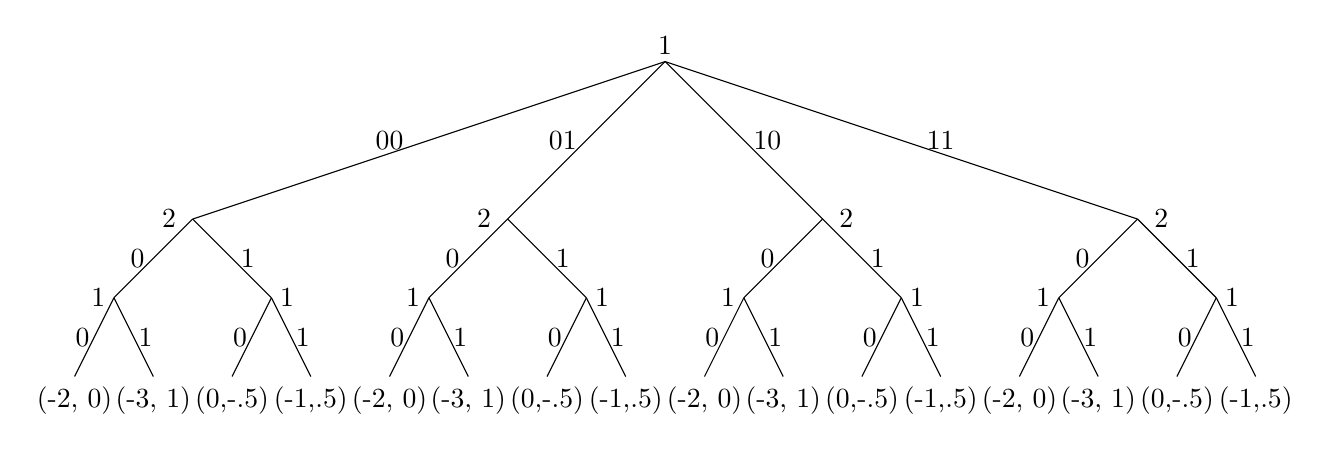
\begin{tikzpicture}
\draw (0.5,1) -- (0,0) node[anchor=north] {(-2, 0)};
\draw (0.5,1) -- (1,0) node[anchor=north] {(-3, 1)};
\draw (2.5,1) -- (2,0) node[anchor=north] {(0,-.5)};
\draw (2.5,1) -- (3,0) node[anchor=north] {(-1,.5)};
\draw (1.5,2) -- (0.5,1);
\draw (1.5,2) -- (2.5,1);
\draw (4.5,1) -- (4,0) node[anchor=north] {(-2, 0)};
\draw (4.5,1) -- (5,0) node[anchor=north] {(-3, 1)};
\draw (6.5,1) -- (6,0) node[anchor=north] {(0,-.5)};
\draw (6.5,1) -- (7,0) node[anchor=north] {(-1,.5)};
\draw (5.5,2) -- (4.5,1);
\draw (5.5,2) -- (6.5,1);
\draw (8.5,1) -- (8,0) node[anchor=north] {(-2, 0)};
\draw (8.5,1) -- (9,0) node[anchor=north] {(-3, 1)};
\draw (10.5,1) -- (10,0) node[anchor=north] {(0,-.5)};
\draw (10.5,1) -- (11,0) node[anchor=north] {(-1,.5)};
\draw (9.5,2) -- (8.5,1);
\draw (9.5,2) -- (10.5,1);
\draw (12.5,1) -- (12,0) node[anchor=north] {(-2, 0)};
\draw (12.5,1) -- (13,0) node[anchor=north] {(-3, 1)};
\draw (14.5,1) -- (14,0) node[anchor=north] {(0,-.5)};
\draw (14.5,1) -- (15,0) node[anchor=north] {(-1,.5)};
\draw (13.5,2) -- (12.5,1);
\draw (13.5,2) -- (14.5,1);
\draw (7.5,4) -- (5.5,2);
\draw (7.5,4) -- (1.5,2);
\draw (7.5,4) -- (9.5,2);
\draw (7.5,4) -- (13.5,2);
\node at (7.5,4.2) {1};
\node at (9.8,2) {2};
\node at (13.8,2) {2};
\node at (5.2,2) {2};
\node at (1.2,2) {2};
\node at (8.8,3) {10};
\node at (11,3) {11};
\node at (6.2,3) {01};
\node at (4,3) {00};
\node at (0.8,1.5) {0};
\node at (2.2,1.5) {1};
\node at (4.8,1.5) {0};
\node at (6.2,1.5) {1};
\node at (8.8,1.5) {0};
\node at (10.2,1.5) {1};
\node at (12.8,1.5) {0};
\node at (14.2,1.5) {1};
\node at (0.3,1) {1};
\node at (2.7,1) {1};
\node at (4.3,1) {1};
\node at (6.7,1) {1};
\node at (8.3,1) {1};
\node at (10.7,1) {1};
\node at (12.3,1) {1};
\node at (14.7,1) {1};
\node at (0.1, 0.5) {0};
\node at (0.9, 0.5) {1};
\node at (2.1, 0.5) {0};
\node at (2.9, 0.5) {1};
\node at (4.1, 0.5) {0};
\node at (4.9, 0.5) {1};
\node at (6.1, 0.5) {0};
\node at (6.9, 0.5) {1};
\node at (8.1, 0.5) {0};
\node at (8.9, 0.5) {1};
\node at (10.1, 0.5) {0};
\node at (10.9, 0.5) {1};
\node at (12.1, 0.5) {0};
\node at (12.9, 0.5) {1};
\node at (14.1, 0.5) {0};
\node at (14.9, 0.5) {1};
\end{tikzpicture}

\paragraph{(b)}
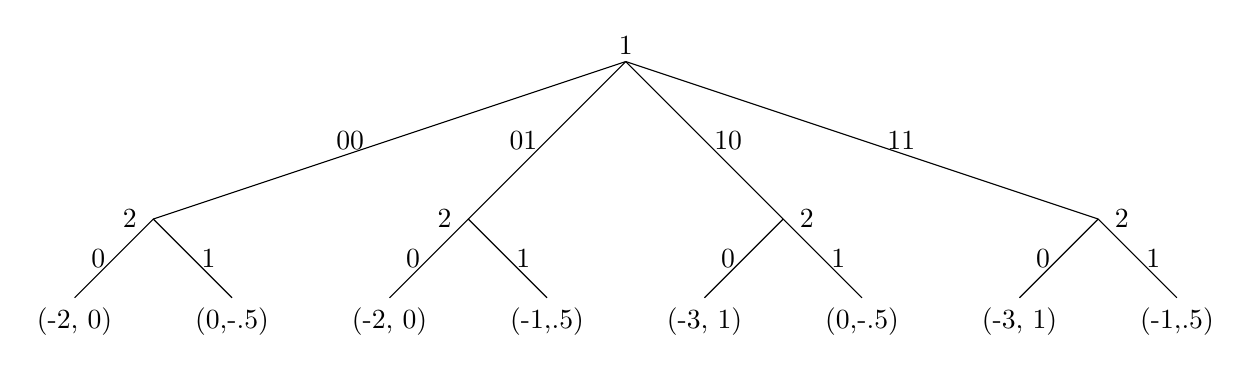
\begin{tikzpicture}
\draw (1.5,2) -- (0.5,1) node[anchor=north] {(-2, 0)};
\draw (1.5,2) -- (2.5,1) node[anchor=north] {(0,-.5)};
\draw (5.5,2) -- (4.5,1) node[anchor=north] {(-2, 0)};
\draw (5.5,2) -- (6.5,1) node[anchor=north] {(-1,.5)};
\draw (9.5,2) -- (8.5,1) node[anchor=north] {(-3, 1)};
\draw (9.5,2) -- (10.5,1) node[anchor=north] {(0,-.5)};
\draw (13.5,2) -- (12.5,1) node[anchor=north] {(-3, 1)};
\draw (13.5,2) -- (14.5,1) node[anchor=north] {(-1,.5)};
\draw (7.5,4) -- (5.5,2);
\draw (7.5,4) -- (1.5,2);
\draw (7.5,4) -- (9.5,2);
\draw (7.5,4) -- (13.5,2);
\node at (7.5,4.2) {1};
\node at (9.8,2) {2};
\node at (13.8,2) {2};
\node at (5.2,2) {2};
\node at (1.2,2) {2};
\node at (8.8,3) {10};
\node at (11,3) {11};
\node at (6.2,3) {01};
\node at (4,3) {00};
\node at (0.8,1.5) {0};
\node at (2.2,1.5) {1};
\node at (4.8,1.5) {0};
\node at (6.2,1.5) {1};
\node at (8.8,1.5) {0};
\node at (10.2,1.5) {1};
\node at (12.8,1.5) {0};
\node at (14.2,1.5) {1};
\end{tikzpicture}

\paragraph{(c)}
The strategies for the government in the first case (nonenforced announcement) are $s_1 \in \{00, 01, 10, 11 \} \times \{ 0, 1 \}^8$. The strategies for the player are $s_2 \in \{ 0, 1 \}^4$. The payoff matrix is then 1024 by 16, and we can populate this from the tree (but it is quite tedious to do so).

If the announcement is enforced, the only government strategies are $\{00, 01, 10, 11 \}$. The player strategies are still $\{ 0, 1 \}^4$. The payoff matrix is now only 4 by 16, and we can populate it from the extensive form game drawn above by tracing the path corresponding to each pair of pure strategy profiles.

\paragraph{(d)}
We use backward induction.

In the first case, where the government is not bound to the announcement, the government is always better off paying transfer 0 regardless of its announcement, because the player's action is locked in. Hence, the player always takes action 0 since taking action 1 with no transfer guarantees payoff $-1/2 < 0$. The government then can make any announcement it wants, or any random announcement according to any distribution over the announcements; the player always then takes action 0 regardless of the announcement and the government pays transfer 0 regardless of the announcement and the action. These are the subgame perfect equilibria in this case.

For the case where the government is bound to the announcement, the player prefers taking action $1$ if and only if the announcement is $01$. Thus, for the government, the payoffs of taking actions $(00, 01, 10, 11)$ are $(-2, -1, -3, -3)$, so the government's strategy is to play $01$, and the player's strategy is $\{ 0, 1, 0, 0 \}$. This is the subgame perfect equilibrium in this case.

\end{document}
	% line of code telling latex that your document is ending. If you leave this out, you'll get an error
